%  Document Config
\documentclass[12pt]{diazessay}



\ksulogo{
    \begin{tikzpicture}[remember picture,overlay]
    \node[anchor=north west,yshift=-1.5pt,xshift=1pt]%
        at (current page.north west)
        {
\includegraphics[height=30mm]{Figures/KSU_logo.png}};
    \end{tikzpicture}
}

\school{King Saud University \\
College of Computer and Information Sciences\\
Computer Science Department}

\title{\textbf{Arabic Text Dialect Recognition}}

\logo{
    \begin{figure}[h]
        % \hskip-3.3cm
        \centering
        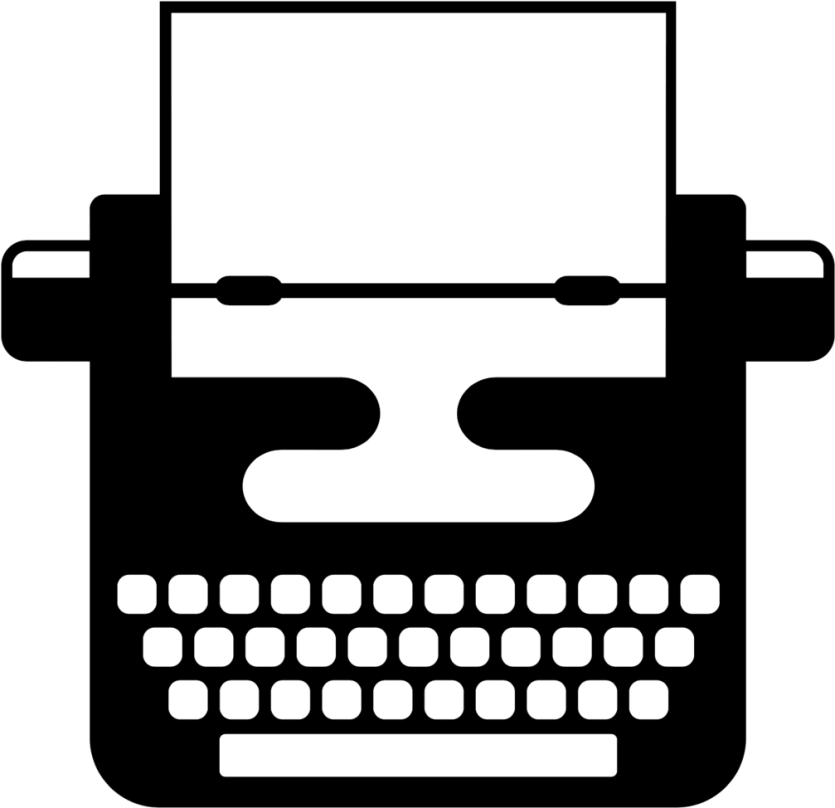
\includegraphics[scale=0.2]{Figures/best_project_logo.png}
    \end{figure}
}

\author{\textbf{Authors} \\ 
Mohand Al-Rasheed \hspace{15pt} 439101298\\
Khalid Albader \hspace{50pt}  439101990\\
Abdulrahman Alshawi \hspace{4pt}  439101980\\
Abdullah Alsuwailem \hspace{11pt}  439101690\\
Musaad Alqubayl \hspace{35pt}  439101884\\
} 
\supervisor{Dr. Nasser Alsadhan}

\date{Research project for the degree of Bachelor in Computer Science \\
First/Second Semester 1443 \\
Autumn/Spring 2021}

% Image config
\usepackage{graphicx}
\graphicspath{ {./Figures/} }

% Code config
\usepackage{listings}
\usepackage{color}

\definecolor{dkgreen}{rgb}{0,0.6,0}
\definecolor{gray}{rgb}{0.5,0.5,0.5}
\definecolor{mauve}{rgb}{0.58,0,0.82}
\definecolor{backcolour}{rgb}{0.99,0.99,0.99}


\lstset{frame=tb,
  language=Python,
  aboveskip=3mm,
  belowskip=3mm,
  showstringspaces=false,
  columns=flexible,
  basicstyle={\small\ttfamily},
  backgroundcolor=\color{backcolour},   
  numbers=left,
  numberstyle=\tiny\color{gray},
  keywordstyle=\color{blue},
  commentstyle=\color{dkgreen},
  stringstyle=\color{mauve},
  breaklines=True,
  breakatwhitespace=true,
  tabsize=1
}


% Section config
\usepackage{titlesec}
\usepackage{hyperref}

\titleclass{\subsubsubsection}{straight}[\subsection]

\newcounter{subsubsubsection}[subsubsection]
\renewcommand\thesubsubsubsection{\thesubsubsection.\arabic{subsubsubsection}}
\renewcommand\theparagraph{\thesubsubsubsection.\arabic{paragraph}} % optional; useful if paragraphs are to be numbered

\titleformat{\subsubsubsection}
  {\normalfont\normalsize\bfseries}{\thesubsubsubsection}{1em}{}
\titlespacing*{\subsubsubsection}
{0pt}{3.25ex plus 1ex minus .2ex}{1.5ex plus .2ex}

\makeatletter
\renewcommand\paragraph{\@startsection{paragraph}{5}{\z@}%
  {3.25ex \@plus1ex \@minus.2ex}%
  {-1em}%
  {\normalfont\normalsize\bfseries}}
\renewcommand\subparagraph{\@startsection{subparagraph}{6}{\parindent}%
  {3.25ex \@plus1ex \@minus .2ex}%
  {-1em}%
  {\normalfont\normalsize\bfseries}}
\def\toclevel@subsubsubsection{4}
\def\toclevel@paragraph{5}
\def\toclevel@paragraph{6}
\def\l@subsubsubsection{\@dottedtocline{4}{7em}{4em}}
\def\l@paragraph{\@dottedtocline{5}{10em}{5em}}
\def\l@subparagraph{\@dottedtocline{6}{14em}{6em}}
\makeatother

\setcounter{secnumdepth}{4}
\setcounter{tocdepth}{4}


\begin{document}


\maketitle 


%----------------------------------------------------------------------------------------
%	ESSAY BODY
%----------------------------------------------------------------------------------------

\tableofcontents

\cleardoublepage

\addcontentsline{toc}{section}{Acknowledgements}
\section*{Acknowledgements}
We would like to express our great gratitude to Dr. Nasser Alsadhan for his valuable suggestions. and his aid throughout the writing of this report. His willingness to give his time so generously has been very much appreciated.

\addcontentsline{toc}{section}{English Abstract}
\section*{English Abstract}
The Arabic language is one of the oldest languages widely used today, and as a result of that, many Arabic speaking regions have formed dialects exclusive to their own. For example, many countries surrounding the Arabic Gulf have formed a dialect different to countries in the Levantine region. We intend on identifying and systematically determining the dialect of a piece of text. 

 This research has many applications in Arabic text analysis, such as helping in identifying the regions customers most often come from by analyzing a product’s reviews and comments and breaking them down by region, which provides useful intel for a business. It also helps in narrowing the nationality of an anonymous writer of a piece of text by predicting their region.
One of the major challenges in dialect recognition is dividing data into classes of dialects. Saudi Arabia and the UAE have dialects that differ widely from each other when solely considered, though they feel very similar in comparison to a Levantine dialect. The researchers will determine a classification easy enough for a machine to detect, but sophisticated enough to be useful. 

We intend to build a machine learning powered classifier that distinguishes between a set number of different Arabic dialects (e.g. Egyptian, Levantine, Gulf, etc.) when given a piece of text. We’ll use state of the art technologies in the field of NLP (natural language processing) in order to train an effective classifier that understands the differences between dialects.


\addcontentsline{toc}{section}{Arabic Abstract}
\section*{Arabic Abstract}
\begin{RLtext}
اللغة العربية من أقدم اللغات المستخدمة بكثرة حاليا، ونتيجة لذلك، الكثير من المناطق المتحدثة للعربية أنشأت لهجات مخصصة بمناطقهم. فعلى سبيل المثال، الكثير من المناطق المجاورة للخليج العربي تتحدث لهجة مختلفة بشدة عن لهجات المناطق الشامية. يعتزم الباحثون على أتمتة عملية التعرف على اللهجات من خلال تحليل قطعة من النص.

البحث له العديد من التطبيقات، وأهمها هو في تحليل النصوص العربية، فمثلا استخدامه في التعرف على مناطق عملاء جهة معينة عن طريق تحليل التقاييم والتعليقات المضافة على منتجاتهم، مما يمكن الجهة على التعرف على عملائهم بشكل أدق. كذلك يمكن استخدامه للتنبؤ بمنشأ مرسل رسالة مجهولة عن طريق التعرف على منطقة انتمائه.

من أهم التحديات في تصنيف اللهجات هي تقسيم البيانات لأصناف من اللهجات. فعلى سبيل المثال، المملكة العربية السعودية والإمارات العربية المتحدة يتحدثون بلهجات مختلفة إذا حصرنا النظر عليهم، ولكن يشبهون بعض حين تتم مقارنتهم مع اللهجات الشامية. سيختار الباحثون مجموعة مناسبة من اللهجات حيث تكون سهلة للنظام في التعرف عليها، ولكن معقدة كفاية لكي تكون مفيدة.

في هذا المشروع ننوي بناء مصنف (\LR{classifier}) مدعوم بتقنيات تعلم الآلة لكي يصنف ما بين مجموعة من اللهجات المحددة (مثل اللهجة المصرية، والشامية، والخليجية، وغيرها) إذا أعطي قطعة من النص. سيستخدم الباحثون أحدث التقنيات في مجال تحليل اللغات الطبيعية (\LR{NLP}) لكي يدربوا مصنف فعال، يفرق بين اللهجات العربية.
\end{RLtext}


\section{Introduction}
    As languages develop across regions far apart from each other dialects begin to take shape, machine learning researchers became interested in classifying text in some language to it's proper dialect. This is because its connected to more insightful text analysis.
    
    A dialect is the variation of a language in grammar, pronunciation and vocabulary. Every individual has their own way of talking that is affected by dialect, accent, background and many other factors\cite{10.5555/2126240}. The Arabic language has a variety of dialects throughout the Arabic world, dialects could differ not only across countries but also in the same country or even city. Arabic dialects differ from one another in pronunciation and vocabulary, different dialects have different words or different variations of a word that could refer to the same meaning, which sometimes make it a bit difficult to understand each other, and it can make it harder for non-Arabic speakers who are trying to learn Arabic.
    
    Machine learning is a branch of artificial intelligence (AI) and computer science which focuses on the use of data and algorithms to imitate the way that humans learn, gradually improving its accuracy\cite{ibm_cloud_education_2020}. It is a rapidly growing field, many countries are racing each other to adapt machine learning technologies and develop smart and automated systems, applications, and adapt them into our daily lives as well as numerous varieties of fields that could benefit from them. Natural language processing, abbreviated as \textit{NLP} is a branch of machine learning that is primarily focused on analyzing text. Numerous companies are racing to develop programs that utilize NLP to analyze user behaviour. One of the difficulties facing companies developing using NLP for Arabic speakers is the numerous varieties of dialects in Arabic.


    \subsection{Problem statement}
    
    Dialects are formed mainly due to regional separation between the Arab world. This separation reduces interaction between different regions, and as a result of that, many Arabic speaking regions have formed dialects exclusive to their own. For example, many countries surrounding the Arabic Gulf have formed a dialect different to countries in the Levantine region. The research’s main problem is how to identify and predict dialect types from written text.

 
    \begin{figure}[h]
        % \hskip-3.3cm
        \centering
        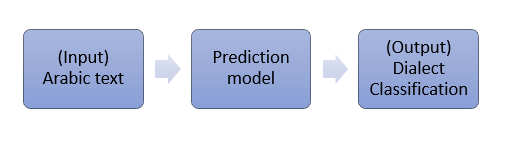
\includegraphics[scale=0.7]{Figures/problem_statment.png}
        \caption{Illustration of the problem}
        \label{fig:cmp}
    \end{figure}
        
    
    \subsection{Goals and objectives}
    
    The goal of this research is to analyze and understand Arabic text to classify the dialect of any piece of Arabic text.
    The objective to implement the most appropriate state of the art NLP model that helps in achieving the best possible accuracy which correlates to correctly classifying what dialect the text is from.

    \subsection{Proposed Solution}
    This research will contribute in solving Arabic dialect detection by using one of the latest advancements in the field of natural language processing.
    
    
    \subsection{Research scope}
    The scope of this research is mainly focused about analyzing, preprocessing and modeling a state of the art NLP model to classify Arabic text into a set of dialects. 


\section{Background}


    \subsection{Natural language processing}
        “Natural Language Processing is a theoretically motivated range of computational techniques for
        analyzing and representing naturally occurring texts at one or more levels of linguistic analysis for the purpose of achieving human-like language processing for a range of tasks or applications.” \cite{natural_language_processing_book}. The field of NLP is an active area of research and development solely for the purpose of computerizing the process of analyzing written/spoken text in a human-like way.
        
        In recent years NLP has become an essential part for many technologies that are relevant today. Companies are taking advantage of the abundance of data that is flooding the internet every day and are developing numerous NLP technologies and applications that we use everyday.
        
        Human languages are surprisingly complex and ambiguous in nature, there are languages that are easier to process for computers than others due to various reasons, such as English and French compared to Arabic and Chinese. However, there has been continuous advancements done on computational techniques that will try to solve challenges around NLP.
    
        
        \subsubsection{Preprocessing}
            Preprocessing refers to the manipulation of raw data to format it in a way so that is easier for computers to process and analyze. It is a technique that is crucial for any NLP task to perform well, it can directly impact the accuracy and performance of any kind of task performed on it. It is the first step taken for any NLP task. Some operations of preprocessing include, \emph{normalization} of data, \emph{segmentation} of data, \emph{tokenization} of text, \emph{stemming} of words and \emph{noise removal}. When dealing with Arabic text usually the first step is filtering out non-Arabic content from text especially when you are getting the content from social media.


            \subsubsubsection{Tokenization}
            Tokenization is the process of breaking down sentences into smaller components such as words called tokens to make it analyzable for computers, it is an important operation in preprocessing text for any NLP task. There are several methods of performing tokenization, such as white tokenization, subword tokenization. White space tokenization breaks sentences into words that we call tokens, while this is useful for languages like English and French, it is needed to perform some additional steps for languages like Chinese and Japanese where words are not separated by spaces. While subword tokenization breaks down words into different tokens, so for example, "Unfriendly" is broken down to "Un", "friend" and "ly" \cite{subword_tokenization}
            
            Tokenization also has limitations for the Arabic language, owing to the complexity of the language, words like "\RL{عقد}" and "\RL{جد}" depending on the context or pronunciation could lead to different meanings, also the difference between spoken language in news and everyday life, and not just in Arabic this is also true for most languages, and that is one of the challenges of tokenization.
    
            
            \subsubsubsection{Word embedding}
            \begin{figure}[h]
                % \hskip-3.3cm
                \centering
                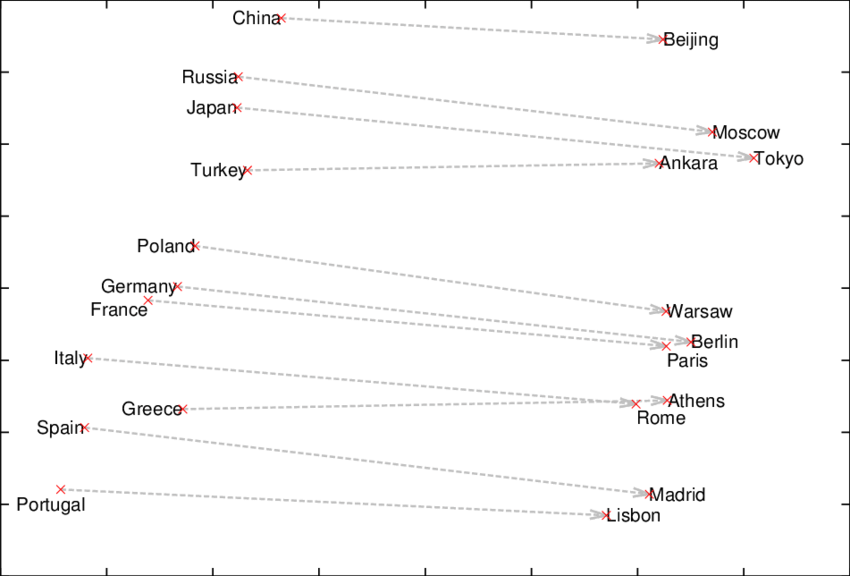
\includegraphics[scale=0.42]{Figures/embeddings_fig.png}
                \caption{Country and capital vectors projected by PCA \cite{PCA_article}}
                \label{fig:wordembedding}
            \end{figure}
            
            Computers can’t understand natural language, so in order to make computers understand it we have to create a representation for a language that a computer can process, and that is what word embedding do. Word embedding is a term used for the representation of words for text analysis, typically in the form of a real-valued vector that encodes the meaning of the word such that the words that are closer in the vector space are expected to be similar in meaning \cite{jurafsky_martin_2000}. There are several word embedding models, and generally all models share the concept of context to determine how close are words to each other, “You shall know a word by the company it keeps!” (Firth, J. R. 1957:11). Figure \ref{fig:wordembedding} shows a model that learnt the relationships between countries and their capitals without information of what a capital city means
    
        
    \subsection{Neural networks}
    
    
        \subsubsection{What are neural networks}
        Neural networks are sub-field of machine learning, and also the parent field of deep learning. Neural networks are made up of layers of neurons and work like interconnected nodes inspired by the neurons inside the brain. By taking in data, they are able to recognize hidden patterns and and correlations in unprocessed data and use said patterns to cluster, classify and predict the data, among other applications. Unlike other machine learning model, neural networks with 
        
        Neural networks layers consist of:
        \begin{enumerate}
            \item Input layer: takes the initial data.
            \item Hidden layer(s): a layer, or more, placed between input and output which captures the non-linearity of the data.
            \item Output layer: produce the outcome of the prediction.
        \end{enumerate}
        
        \begin{figure}[h]
            % \hskip-3.3cm
            \centering
            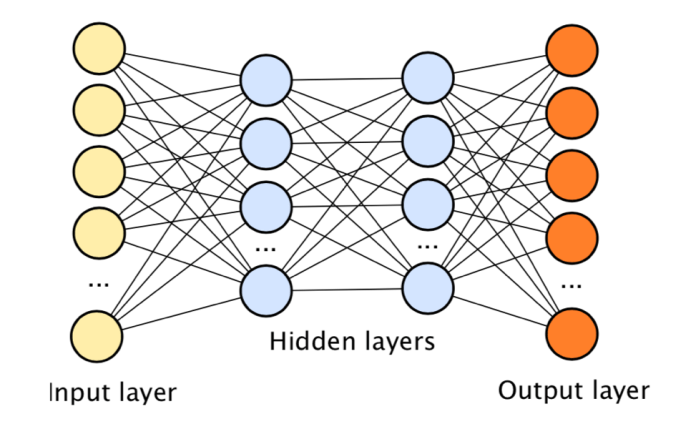
\includegraphics[scale=0.5]{Figures/neural networks.png}
            \caption{Neural networks architecture \cite{marcus2018deep}}
            \label{fig:cmp}
        \end{figure}
        
        Neural networks also are ideally fitted to assist humans solve complicated issues in real-life situations. They can examine and model the relationships among inputs and outputs which can be nonlinear and complicated; make generalizations and inferences; monitor hidden relationships, styles and predictions. Also, neural networks can enhance choice methods for natural language processing.
        
        
        \subsubsection{Neural networks in natural language processing}
        Neural networks are now prevelant in NLP such text classification (which is the objective of this research), machine translation, semantic parsing, which extracts useful bits of information in a large text, and many many more.
        
        % A great amount of NLP based applications (e.g., sentiment analysis, text classification, etc...) depend on language models. which define a probability distribution over sequences of words, characters or bytes in a natural language Different pre-trained language models have been proposed to address various domain-specific problems, one such model is BERT. 
        %%%%%%%%%%%%%%%%%%%%% Great summary of language representation, I think we might need to write it in the methodology section

        
        \subsubsection{Transformers}
        

    \subsection{Dialect prediction approaches}
        One can approach the problem of dialect prediction in a number of ways, We will define and discuss some different dialect recognition approaches that differ in how they work.

        
        \subsubsection{Rule-Based approach}
        Rule-based approach relies in written curated instructions made by humans to identify selected parts of the text that match a certain logic or found in dictionaries, a popular example in text classifications is to count the number of each word that relate to a category and the highest word count for a category classifies the text in that category. 
        
        Another example would be the Lexical Functional Grammar (LFG). "The LFG system incorporates a richly annotated lexicon containing functional and semantic information."\cite{hassan_2010}.

        
        \subsubsection{Automatic Machine-learning approach} \label{txt:simple_voting}
        Dialect recognition automatic approach is based in machine learning, where it tries to build a statistical model that learns by analysing the training data after choosing an appropriate algorithm and applying NLP techniques, very famous algorithms in text classification would be support vector machines, naïve bayes and deep learning.
        
        
        \subsubsection{Hybrid approach}
        "Hybrid systems combine a machine learning-trained base classifier with a rule-based system, used to further improve the results. These hybrid systems can be easily fine-tuned by adding specific rules for those conflicting tags that haven’t been correctly modeled by the base classifier."\cite{monkey_learn_NLP}
        
        
    \subsection{Performance metrics}
    In binary\footnote{We can use precision and recall in multiclass classification by considering one class, \(A\), at a time and lumping all other classes as \(not A\)} classification problems we can test the performance of out results by matching the output of our model, the predicted label, to the real label in our data. This measure is known as the \emph{accuracy} of our model according to the data. However there are more sophisticated measures that one can observe. We'll talk about two of those measure, mainly \emph{precision} and \emph{recall}.
    
    First, we must define 4 quantities, \textbf{True Positive}, abbreviated \(TP\) consists of \emph{true} which refers to the data being belongs to class 1, while \emph{positive} refers to the model's prediction being class 1. And \textbf{False Negative} is similar to \(TP\) but in the context of class 0. We can mix and match \(T\), \(F\), \(P\) and \(N\) to get 4 different quantities.
    
    Here we define precision and recall in the following way:
    
    \[Precision = TP / (TP + FP)\]
    
    \[Recall = TP / (TP + FN)\]
    
    We can tweak the model's threshold of classification in order to achieve a different Precision and Recall metrics

    % \subsection{Python} % Lets talk about his in the methodology 
    % \subsection{Transformers library}

\section{Literature review}
The discussed problem in this research has been tried by many researchers over the years with varying results, in this section we intend to highlight the most important results regarding the Arabic language, the Arabic corpora and dialect classification methods that has been concluded from past research.
    
    
    \subsection{The Arabic language}
    "The Arabic language is a Semitic language originating on the Arabian
    Peninsula, and it is considered one of the major languages in the world. As a
    result of the expansion of Islam from Spain to Persia, the Arabic language is
    spread across many countries." \cite{alshutayri}
        
        
        \subsubsection{Arabic dialects}
        Dividing Arabic into different dialects is not a standardized task as dialects shift and change depending on the time and how much precision we intend to administer in our breakdown. Researchers working on this problem have found various breakdowns that we'll discuss. 
        
        Habash (2010) has suggested the following breakdown, while adding "and should not be taken to mean that all members of any dialect group are completely homogenous linguistically" \cite{habash}.
        \begin{enumerate}
            \item Egyptian Arabic (EGY) which spans Eygpt and Sudan
            \item  Gulf Arabic (GLF) which spans the Arabic peninsula, Habash adds "although there is a wide range of sub-dialects within it." And "Omani Arabic is included some times."
            \item Levantine Arabic (LEV) which spans the Levantine region
            \item "North African (Maghrebi) Arabic (Mag) covers the dialects of Morocco, Algeria, Tunisia and Mauritania. Libyan Arabic is sometimes included." \footnote{Many other researchers abbreviate North African dialects as "NOR"}
            \item "Iraqi Arabic (IRQ) has elements of both Levantine and Gulf"
            \item "Yemenite Arabic (Yem) is often considered its own class"
        \end{enumerate}
        
        \begin{figure}[h]
            % \hskip-3.3cm
            \centering
            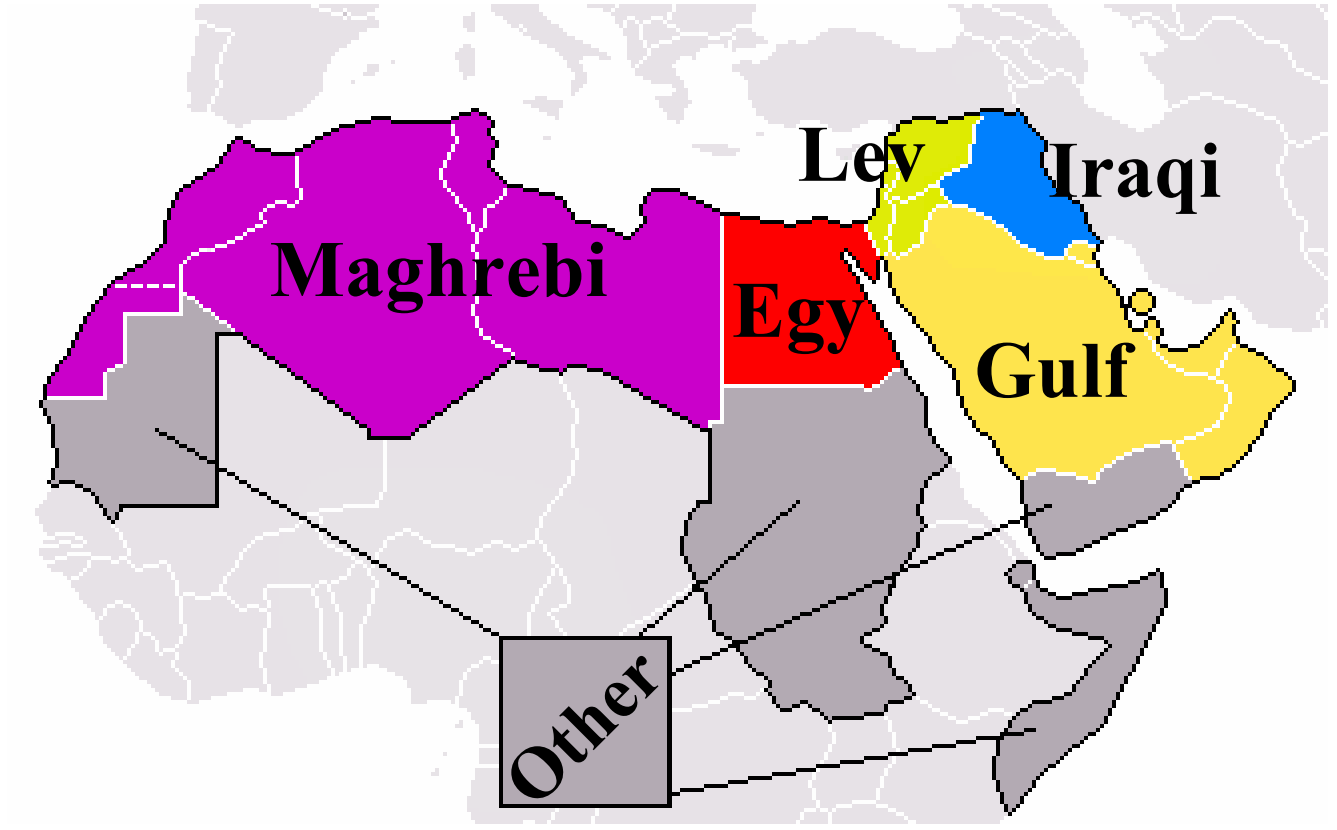
\includegraphics[scale=0.2]{Figures/Zaidan and Burch dialect breakdown.png}
            \caption{Zaidan and Callison-Burch (2011) gave a similar breakdown\cite{zaidan_burch} to Habash's}
            \label{fig:cmp}
        \end{figure}
        
        Alshutayri (2018) also gave a similar breakdown, which is GLF (including Oman), EGY, LEV, NOR (which includes Morocco, Algeria, Tunisia and Libya) and IRQ which we'll be using in this research. Although the breakdown is somewhat general and imprecise, its general enough to be useful in data collection and in classification.
        
        
    \subsection{Existing Arabic text corpora}
    The problem of dialect classification has been studied in the past with many studies building their own corpora, here we'll examine the most prominent corporas.
    
    In 2015 Shoufan and Alameri conducted a literature review, in which they summarised the advancments in NLP for dialectal Arabic\cite{shoufan_alameri_2015_natural} in the following comprehensive table. Bear in mind that the table includes more than text analysis and also includes speech analysis.
    
    \clearpage
    \begin{figure}[h]
        \hskip-3cm
        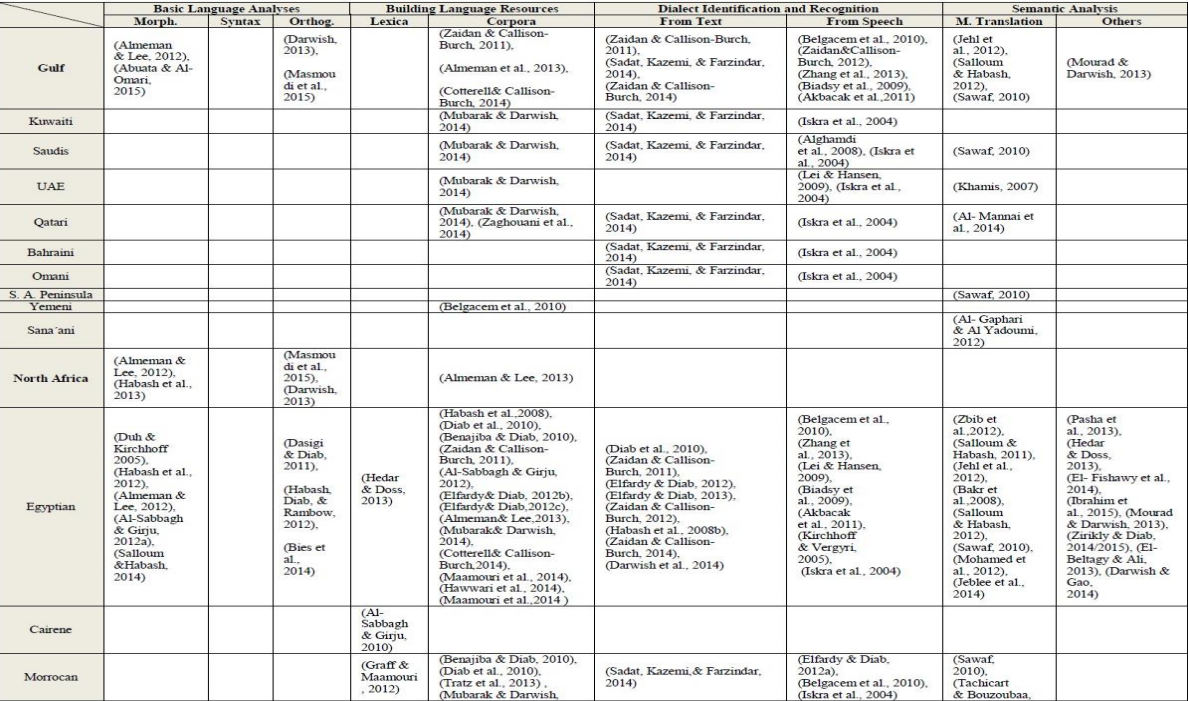
\includegraphics[scale=0.45]{Figures/past_word_1.png}
        \caption{Dialectical Arabic NLP- Literature Overview (Shoufan and Alameri, 2015)}
        \label{fig:cmp}
    \end{figure}
    
    \clearpage
    \begin{figure}[h]
        \hskip-3cm
        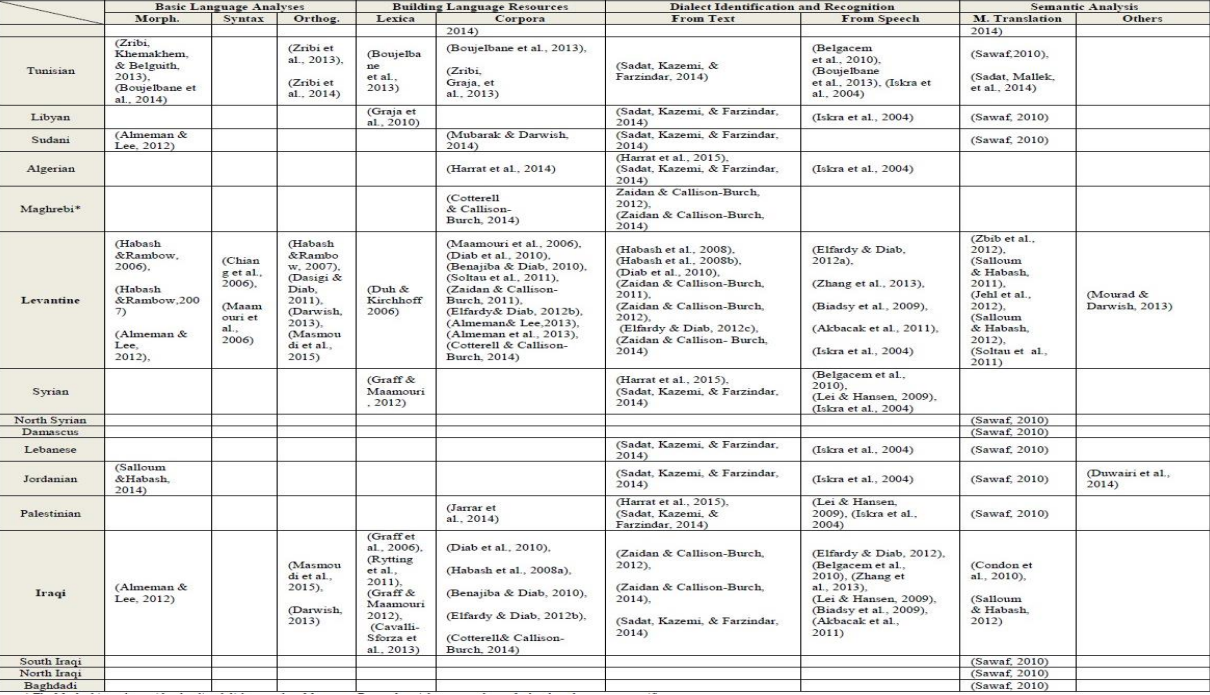
\includegraphics[scale=0.45]{Figures/past_work_2.png}
        \caption{Dialectical Arabic NLP- Literature Overview (Shoufan and Alameri, 2015)}
        \label{fig:cmp}
    \end{figure}
    \clearpage
    
    
    The most prominent corpora collected is the Arabic Online Commentary (AOC) dataset which gathered millions of comments from three newspapers.\cite{zaidan_burch}\label{txt:aoc}
    
    Though the AOC dataset was big enough, it was not annotated fully, which might harm the predicting model's results, so El-Haj et al. (2018) created an annotated dataset built from the AOC dataset alongside North African dialectical data collected from from the Tunisian Arabic Corpus\footnote{http://www.tunisiya.org/}. Then the researchers annoatated the collected data by using Amazon's \emph{Mechanical Turk} (MTURK), which hires online annotators\cite{el_haj_etal_2018_arabic}.
     
    Another improvment of the AOC dataset came from Cotterell, Callison-Burch (2014), in which they extended the AOC newpaper dataset to include about 550K words from 5 newspapers "\textbf{Al-Youm Al-Sabe’}, a Saudi-Arabian newspaper \textbf{Al-Riyadh}, a Jordanian newspaper \textbf{Al-Ghad}, an Algerian newspaper, \textbf{Ech Chorouk El Youmi} and an Iraqi newspaper \textbf{Al-Wefaq}."\cite{cotterell-callison-burch-2014-multi}. As well as 660k words scraped from twitter tweets. After collecting the extended dataset, they manually annotated them using Amazon's Mechnical Turk.
     
    There has been work in using social media as a valid source of dialectic data, creating the SMADC dataset, which scraped and annotated data from Twitter and Facebook\cite{alshutayri_inproceedings}.
    
    Another dataset is the The Dialectal Arabic Tweets (DART), which manually annotated over 25k tweets in Maghrebi, Egyptian, Levantine, Iraqi, and Gulf\cite{alsarsour-etal-2018-dart}
     
     
    \subsection{Dialect classification results}
        There has been many attempts in solving the problem of this research, many of which use similar strategies. In this section we'll review the highlights of past literature's results.
        
        Firstly, Zaidan-Burch (2014), the researchers behind the AOC dataset mentioned in section \ref{txt:aoc}, using "SRILM toolkit to build word trigram models, with modified Kneser-Ney as a smoothing method, and report the results of 10-fold cross validation"\cite{zaidan_burch} have achieved an accuracy of 0.694 at classifying "MSA vs. LEV vs. GLF vs. EGY"\cite{zaidan_burch}.
        
        Cotterell-Burch (2014) have extended the AOC data, also mentioned in section \ref{txt:aoc} and trained using two algorithms, SVM and Naive Bayes using unigram, bigram and trigram features\cite{cotterell-callison-burch-2014-multi}. The results are displayed in figure \ref{fig:extended_aoc_results}
        
        \begin{figure}[h]
            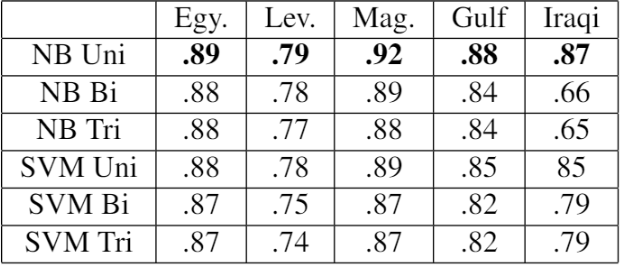
\includegraphics[scale=0.6]{Figures/results_extended_AOC.png}
            \caption{"Experiments on newspaper commentary data (accuracy reported)."\cite{cotterell-callison-burch-2014-multi}}
            \label{fig:extended_aoc_results}
        \end{figure}
        
        Alshutayri used the SMADC dataset to classify dialects to GLF, NOR, LEV, EGY and IRQ. The researcher used Sequential Minimal Optimization (SMO) algorithm with multinomial Naive Bayes (MNB) with different tokenizers, run via the data analysis tool WEKA to achieve an accuracy of 0.6068\cite{alshutayri}.
        
        Alshutayri have also tried lexical methods. One of which is simple voting, which was described in \ref{txt:simple_voting}. Using the SMADC dataset, the researcher achieved an accuracy of 0.6919. The researcher also experimented with weighted voting, filtering based on MSA words and more\cite{alshutayri}.
        
        \begin{figure}[h]
            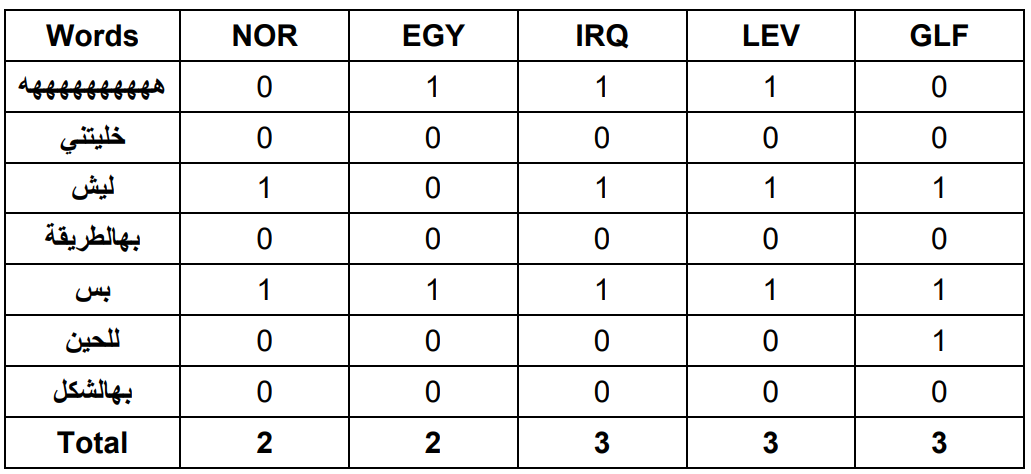
\includegraphics[scale=0.35]{Figures/smadc_simple_voting.png}
            \caption{Simple voting matrix representation of \RL{ههههههههههه خليتني ليش بهالطريقة بس للحين بهالشكل}\cite{alshutayri}}
        \end{figure}
        
        
        \subsubsection{Deep learning dialect classification results}
            Most of the research around dialect classification uses traditional text classification methods and deep learning methods are scarcely used, however, the surge of deep learning research has reinvigorated the interest in deep learning text classification.
            
            Elaraby and Abdul-Mageed (2018) have used many different algorithms including deep learning algorithms such as CNN, CLSTM, LSTM, BiLSTM, BiGRU and Attention BiLSTM which they explain in their paper\cite{elaraby-abdul-mageed-2018-deep} as well as traditional classifiers such as SVMs, Naive Bayes and other.
            
            On the AOC dataset Elaraby and Abdul-Mageed used this dialect split "MSA vs. Egyptian vs. Gulf vs. Levantine" to obtain an accuracy of 0.8245 using the Attention BiLSTM with (Abdul-Mageed, et al.)'s embeddings\cite{elaraby-abdul-mageed-2018-deep}.
            
            It's also noteable that the traditional classifiers won over deep learning classifiers only on the "EGY, GLF, and LEV" three way classification split\cite{elaraby-abdul-mageed-2018-deep}.

\bibliographystyle{plain} % We choose the &quot;plain&quot; reference style
\bibliography{cite.bib} % Entries are in the &quot;refs.bib&quot; file</code></pre>

\end{document}
